\begin{appendix}
\section{Knoten des Legendrepolynoms}

\begin{figure}
  \centering  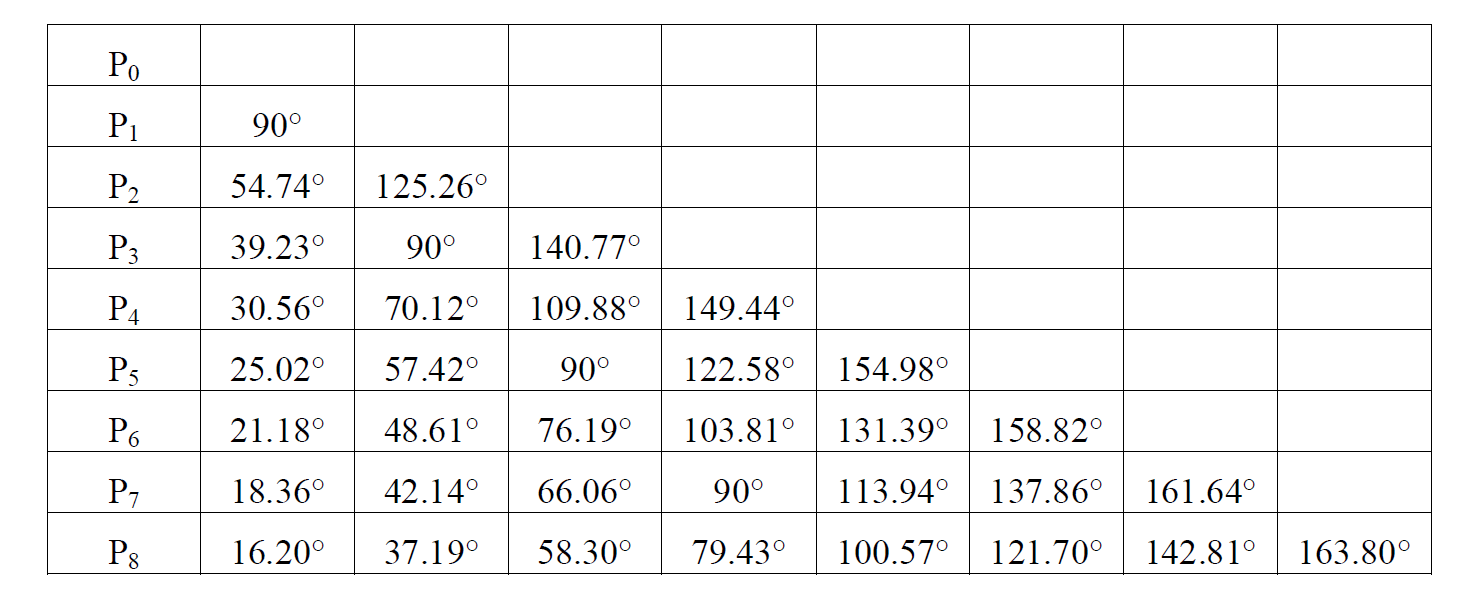
\includegraphics[width=\textwidth]{ressources/WinkelLegendre.png}  \caption{Der Winkel $\Theta$ an den Knoten des Legendrepolynoms $P^{m}_{l}(\cos{(\theta)}) = 0$, \cite{skript}.} \label{fig:Anh1}
\end{figure}
% \newpage
% \begin{figure}
% \includepdf[width=0.9\textwidth, pages={2}]{Bilder/Messdaten.pdf}
% \end{figure}

\end{appendix}
